\chapter{Implementation}
\label{ch:Implementation}

This chapter explores some key concepts about the implementation of the simulation platform that was built. 
All the code and routines that were produced, and that as a whole form the platform have been named PeyeQM.  
In the first section an overview of the Object Oriented Paradigm will be presented to contextualize some of the notions used in further sections. Then we will present a simplified structure of what a Finite Element solver should have, and from that, the implementation of PeyeQM will be treated in a rather simplified form. Finally, a brief explanation of what is Python (the language we used to program) and other two tools is given. The reader is encouraged to see the documentation for routines available online in the following repository \href{https://github.com/bebopsan/peyeQM}.
  
\section{Object Oriented Paradigm}

During developments of FEM software, there have been changes in programming paradigms, from the traditional procedure-oriented to the object-oriented. Being the traditional procedure usually tied to  Fortran and C programming languages, and the object-oriented to higher level languages such as C++, Java, and Python.

Generally speaking, under procedure oriented paradigms when software platforms grow, necessary changes in the code (say, addition of new kinds of elements) require changes in the whole program. Inter dependencies  in the program architecture are often hidden and difficult to determine. Most of the time, in procedure oriented paradigm a high degree of knowledge of the entire program is necessary to modify small routines \cite{Mackerle2004}. Extensibility and flexibility are thus two important qualities that the procedure oriented paradigm lacks. 
Flexibility and abstraction are the keys to manage complexity \cite{Lage1998}, and they are two of the requirements that a FE platform must meet. The following is a list of general requirements that PeyeQM was meant to meet:

\begin{description}
\item[Modularity] Construction of a software by almost independent or loosely coupled components \cite{Lage1998}
\item[Reusability]  The likelihood that a segment of source code can be used again to add new functionalities with slight or no modification. 
\item[Extensibility] A design principle where the implementation takes into consideration future growth.
\item [Multi platform capabilities]  Computing methods and concepts that are implemented and inter-operate on multiple computer platforms \cite{PCMag}.
\item[Readability]  A human judgment of how easy a
text is to understand. ``The readability of a program is related
to its maintainability'' \cite{Raymond2008}.
\end{description}

Now, one programming paradigm that satisfies these requirements is the Object-Oriented Paradigm (OOP). A program implemented under OOP may be viewed as a collection of interacting objects, as opposed to the conventional model, in which a program is seen as a list of tasks (subroutines) to perform \cite{Wikipedia2013}.
The objects that form a program under OOP are representations of things with inherent qualities and attributes. They are capable of receiving messages, processing (or storing) data, and sending messages to other objects. \textbf{Modularity} is then obtained by abstracting the process of a FE computation as the interaction between a set of objects, each of which represents a stage or process. \textbf{Reusability} and \textbf{extensibility} are a consequence of the objects being independent one of the other, defining their relations as parsing of messages that are sufficiently general, allows programers that work on different sections of the code to treat objects they are not working on as \href{http://en.wikipedia.org/wiki/Black_box}{\textbf{black boxes}}. Now, as long as the message doesn't change, work on one object does not affect other parts of the program, so new functionalities can be easily added. In order to achieve a good implementation of a OOP program one needs to start from the beginning with a good idea of the general structure of objects and their interrelations, so that the strengths of OOP qualities get well-exploited. 
The main characteristics of Object Oriented programming are:

\begin{description}
\item[Data abstraction] In OOP data abstraction is obtained by definition of classes. A class is the set of common attributes that a general object of a certain kind or \textit{class} has. For example, ``Banana'' class would represent the properties and functionality of bananas in general, such as being edible, or having potassium. Usage of data abstraction allows us to generalize the behavior of objects independently of what is their current state (name, value of its attributes).  
\item[Encapsulation] Is understood as the possibility of a language or paradigm of bundling data with the methods (or functions) that act on it, or have to do with it. So, in OOP objects not only contain information, but are capable of performing tasks because they have the functions for that built in their definition. In our example a Banana of Class Banana not only would have potassium but would also have the possibility of making someone fall if step upon.
\item[Inheritance] In OOP is the possibility of the paradigm to define classes of classes. Something like nesting of abstractions. For example a Banana is a class derived from a more general abstraction known as ``Fruit'', and has things (grows from trees)\note[NGZ]{Desde cu\'ando los bananos crecen en \'arboles?} in common with other Fruit classes such as ``Orange'' and ``Apple''.
\item[Polymorphism] is a characteristic of operators that can act over objects without caring about its precise type. OOP allows the overloading of operators such that depending on the definitions of the class, certain operators perform different actions. For example in Python the $+$ sign is polymorphic in the sense that it can add integers, if acting on integers, and concatenate strings if acting on strings.
\end{description}

All of this characteristics make the Object Oriented Paradigm a suitable framework from which to design FE software platforms such as PeyeQM according to the requirements listed above.

\section{General stages in a simulation}

There are three main stages in a finite element algorithm:

\begin{enumerate}
\item Pre-Processing
\item Analysis
\item Post-Processing
\end{enumerate}

With the aim of focusing on problem solving and reduce coding of a very complicated platform, we have designed PeyeQM to perform only the critical parts of these stages and have resorted to external software to do Meshing and visualization as illustrated in figure \ref{fig:stages_comp}. 
%
\begin{figure}
\centering
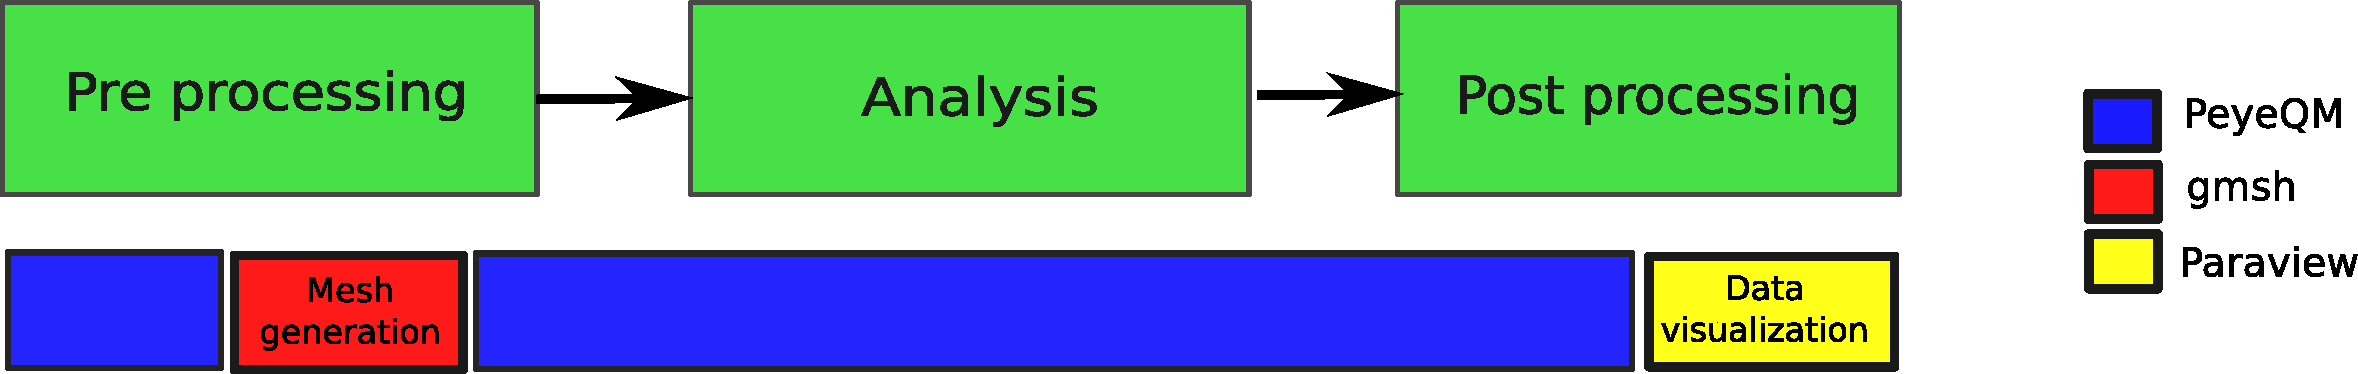
\includegraphics[scale=.3]{./img/stages_comparison.pdf}
\caption{Representation of how much of the simulation process is performed by using PeyeQM's routines.}
\label{fig:stages_comp}
\end{figure}  
%
The following is a brief description of what is done in each stage:

\subsection{Pre-Processing}
Pre-Processing is the stage where we describe the problem that will be solved, in terms that are readily interpreted by the analysis (processing) stage. In other words, is what we need to do before solving. Comparing simulating to cooking this would be the moment when we choose and chop the ingredients as well as heating the stove. Preparing the ingredients in FEM means to:
\begin{itemize}
\item Define the geometry or domain of the simulation, with its regions and associated materials.
\item Define what kind of physics rule the problem, and what kind of solution we want.
\item Discretize or divide the domain in nodes and elements by using a meshing algorithm. 
\item Set boundary and initial conditions.
\item Based on the physics of the problem, build a system of equations that relate all of the above.
\end{itemize} 
 
\subsection{Analysis}
In the Processing or Analysis stage, we take the system of equations that has been constructed in the first stage and solve it using the respective numerical methods. If we have a stationary problem then  we have to solve a system of linear equations, if it is an eigenvalue problem, then we have find the eigenvalues and vectors of a certain matrix, and if it is an explicit solution then we must loop over unknowns assigning values. All in all, what we will do in this stage is the equivalent to the actual cooking of the ingredients. 

\subsection{Post-Processing}
Post processing, is to get the solution produced by the solver and serve it in a portioned and digestible way. In this step we will generally produce graphs, plots, and animations that represent the characteristic of the simulated phenomenon. If Pre-Processing was a sort of codification from human language to algorithm, then Post-Processing is a way of de-codification, from numbers to ``human''.

\section{Classes, Diagrams and flow charts of PeyeQM}
PeyeQM follows this basic Scheme but divides the Pre-Processing stage in two, one part is the assembling of the simulation and the second is the codification or interpretation of that simulation. Figure \ref{fig:stages_2} shows the interpretation that we have made of the  steps to follow.
\begin{figure}[h]
\centering
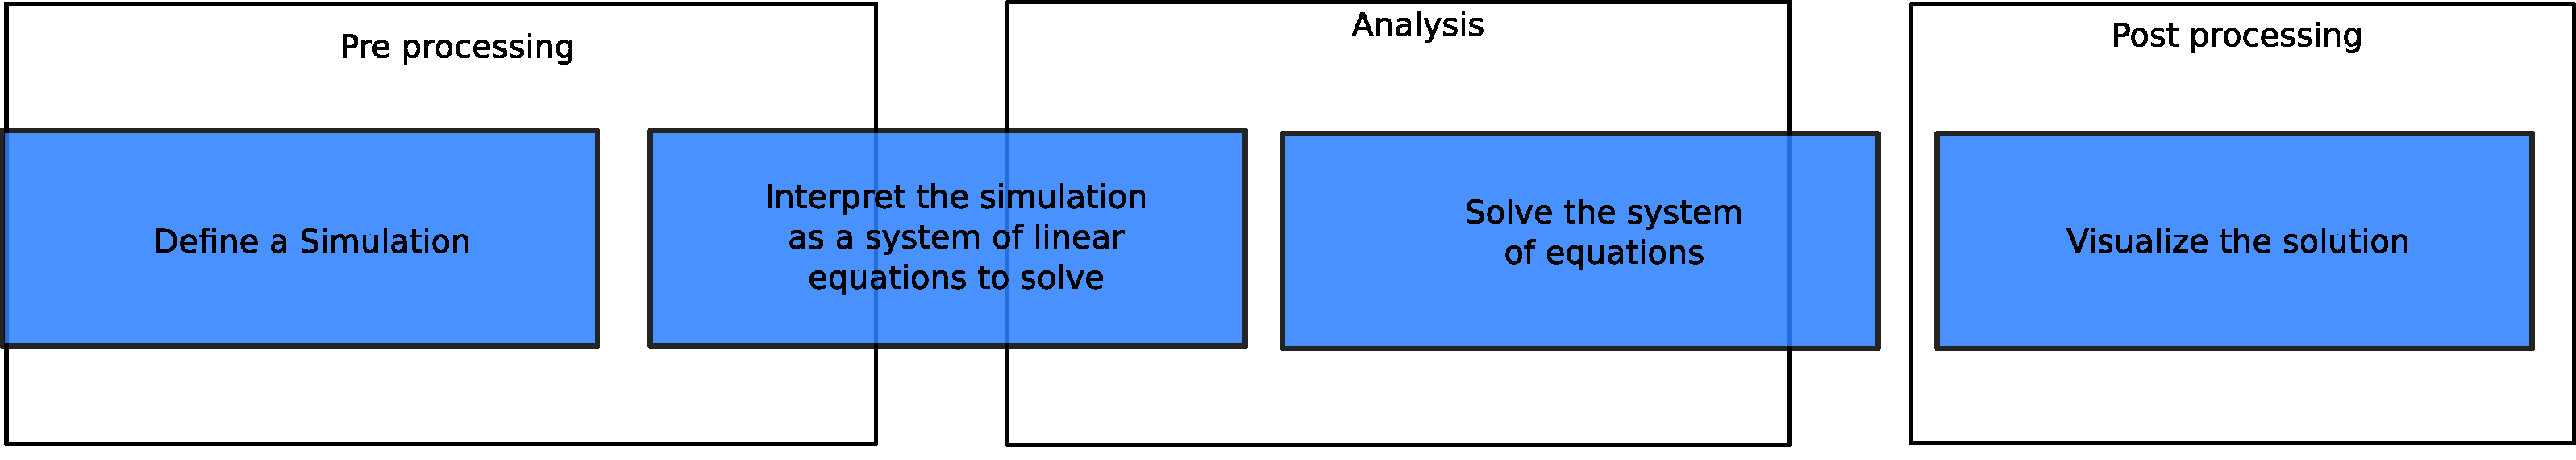
\includegraphics[scale=0.3]{./img/stages_abstract.pdf}
\caption{Diagram of general simulation stages as abstracted by PeyeQM.}
\label{fig:stages_2}
\end{figure}

The way in which we formulated the program in the context of OOP was to use three main classes that deal with the flow of chart \ref{fig:stages_2}.
\begin{itemize}
\item A \textit{Simulation} class,
\item \textit{Interpreter} class, and
\item \textit{Solver} class.
\end{itemize}
In that way, a simulation can interpreted as a kind of conversation between the user and members (instances or objects) of those classes. The first part of that conversation would be the user telling what he wants to a member of class \textit{Simulation}. Doing so the object ``simulation'' gets informed of the parameters needed to solve the problem.  The solver however does not understand either human language or the simulation language, and it needs some intermediary to hear what the simulation has to say and translate it as systems of equations which are its language. This new character is called the Interpreter and is a member of class \textit{Interpreter}. The interpreter is capable of reading the simulation and depending on the kind of physical problem, conditions and domain, will build the matrices and vectors mentioned in chapter \ref{ch:Finite_element_method}, and assemble them in the form of an equation. At this point of the conversation, the Solver, who is a member of class \textit{Solver} will listen to the interpreter and proceed to diligently solve the problem. Whenever the solution is ready it will then return the solution as a file that is in a predefined format, this file will then be passed to the Post-Processor, who will paint the solution for the user closing the loop of this conversation\footnote{It is important to remember now that we are using an external tool called Paraview for the visualization of data.}. 

A diagram showing the main classes that form a Simulation in PeyeQM can be seen in figure \ref{fig:classes}.

\begin{figure}
\centering
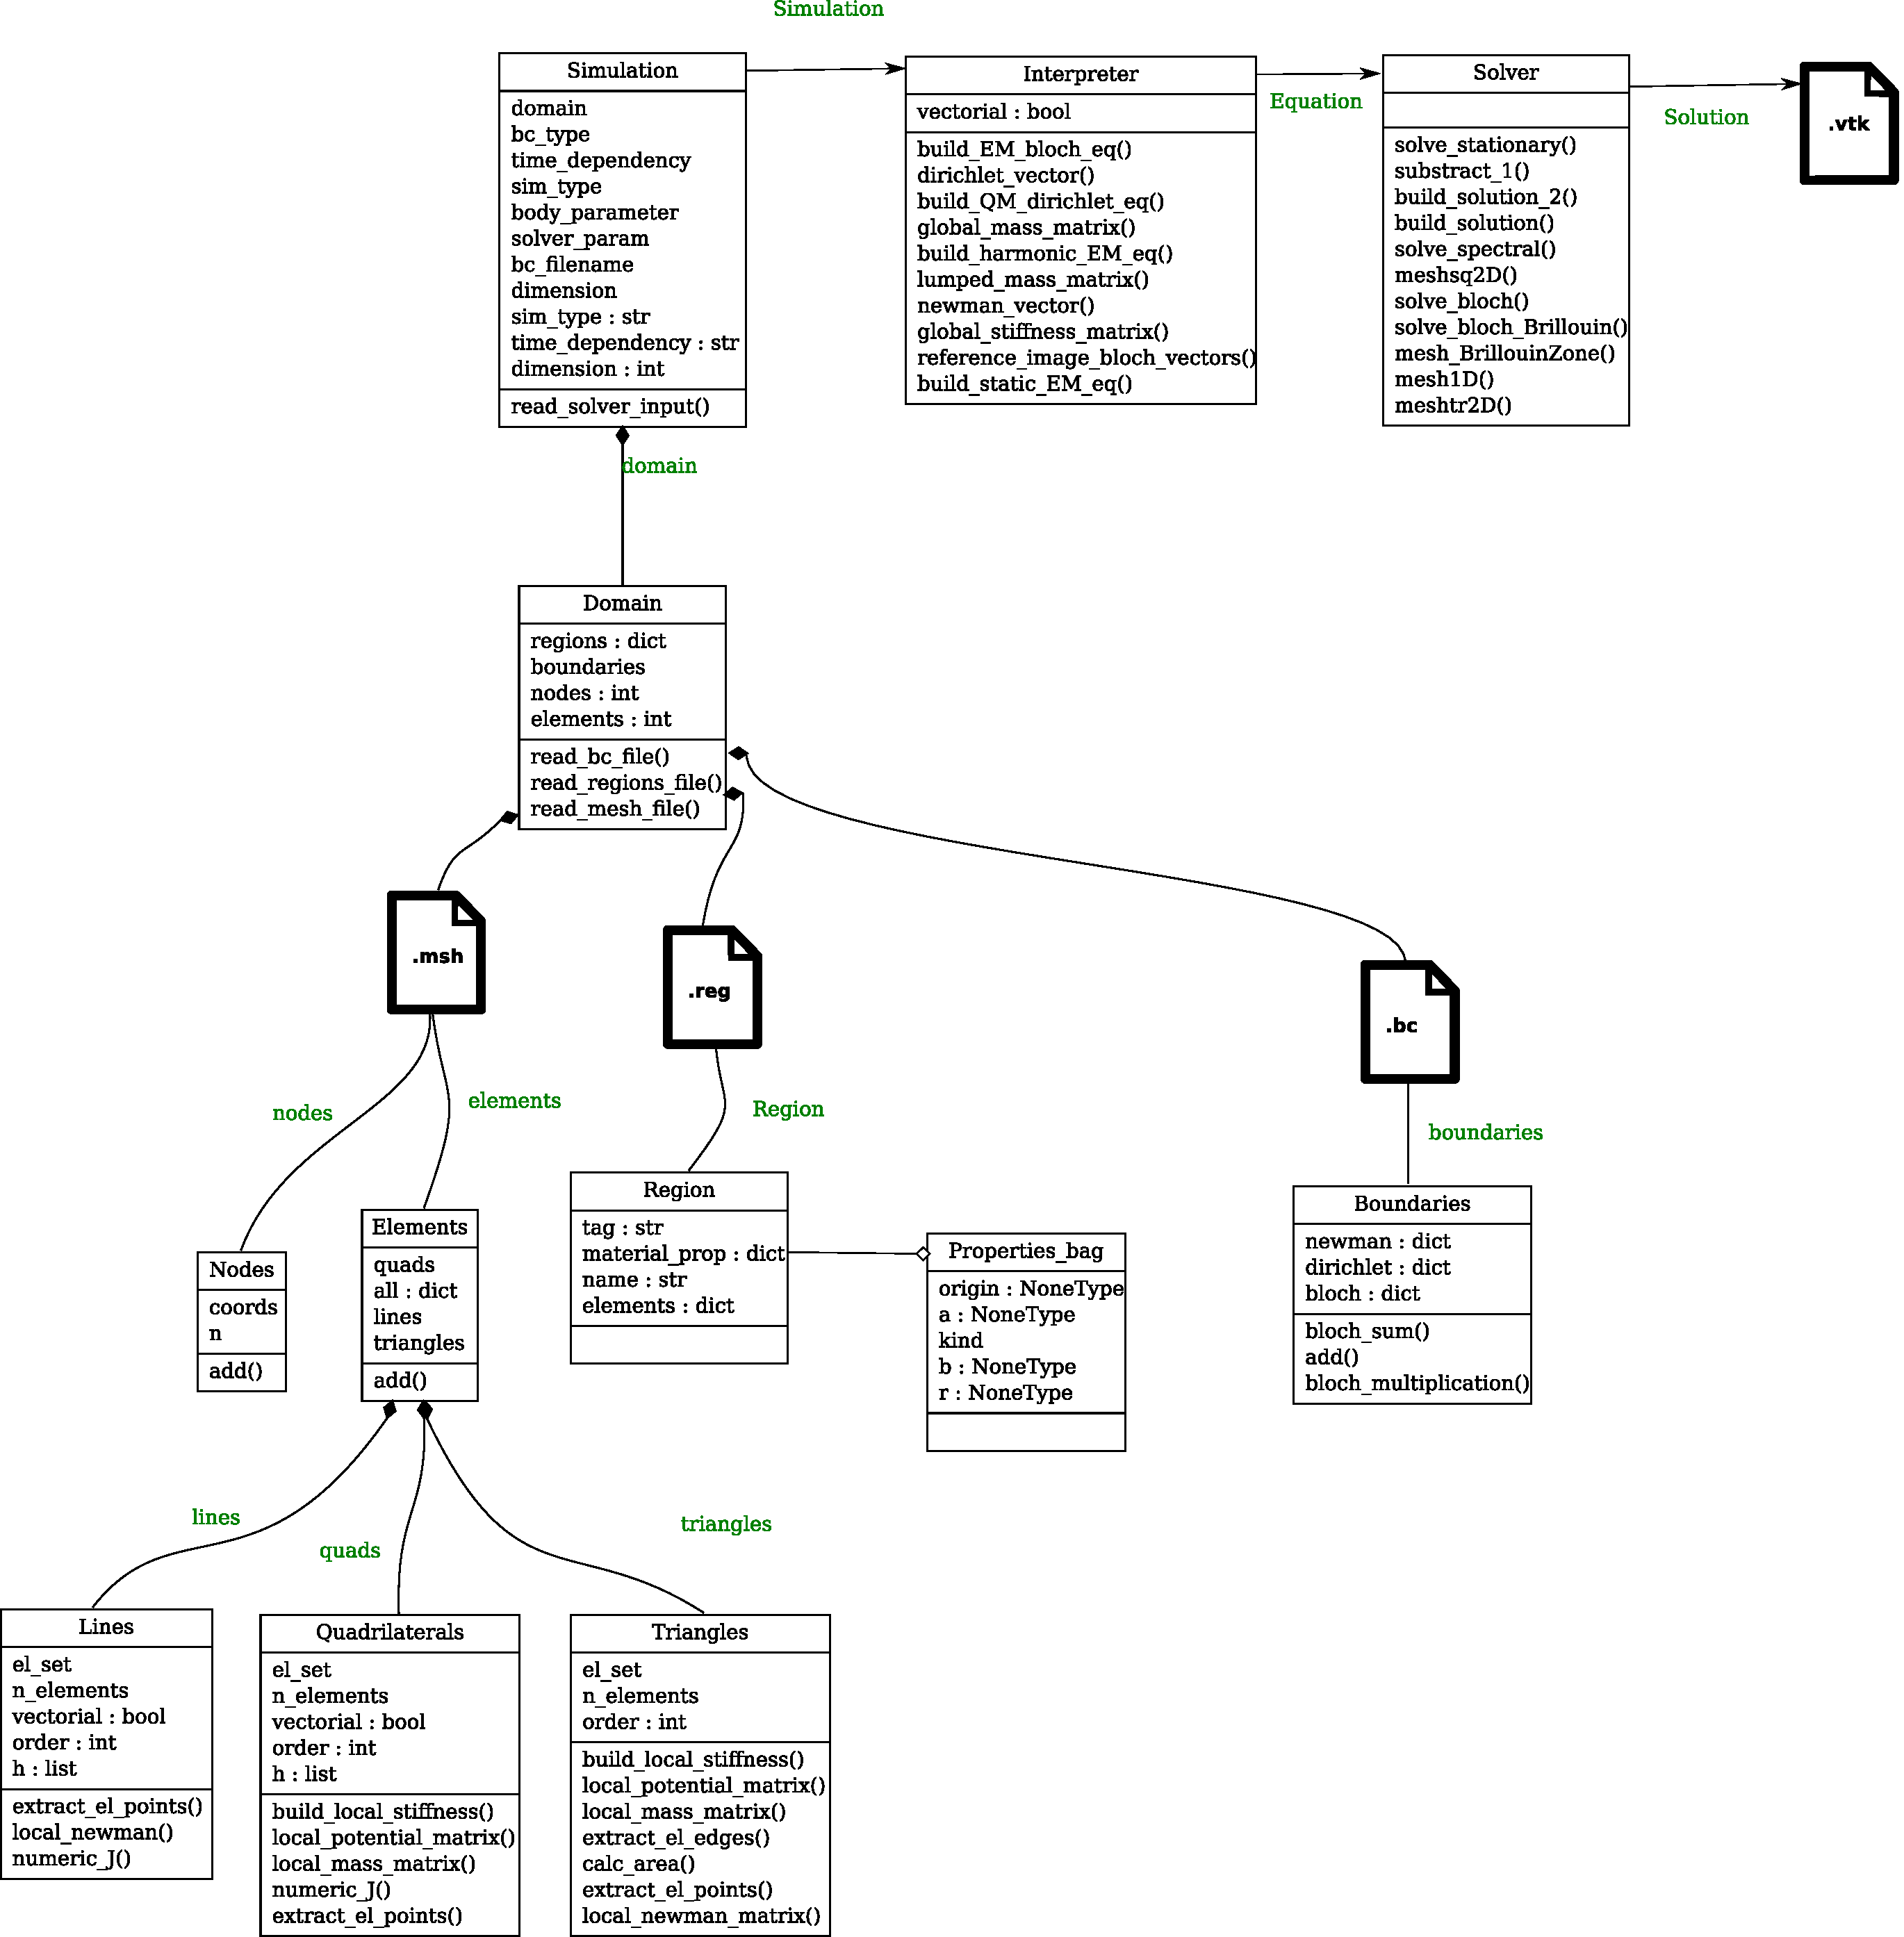
\includegraphics[scale=0.35]{./img/class_diagram.pdf}
\caption{This diagram shows the main classes defined PeyeQM. Classes that are called by a method are connected with lines that end with a black diamonds, and classes that are attributes of other classes are connected by white diamonds.}
\label{fig:classes}
\end{figure}

\section{PeyeQM usage}
The best way to explain how to use the platform is with an example. As it is right now, the platform works by using Python scripts\footnote{Programs that can interpret and automate the execution of tasks which could alternatively be executed one-by-one by a human operator.} that can be run by a computer that has Python console installed. In this section we will explain each line of a script  file (called \href{https://github.com/bebopsan/peyeQM/blob/Depuration/Lib/OOPyQM/Examples/Square\%20waveguide/Waveguide.py}{Waveguide.py}) used to simulate the field inside a wave guide\footnote{A proper explanation of what is a waveguide is made in chapter \ref{ch:Results}}, hoping that with that the reader gets an idea of how to use the libraries and encouraging him-her to explore the examples that have been uploaded in the repository. 

Starting from the first two lines we define what to use in order to execute the file and the kind of coding:
\begin{python}[language=python]
#!/usr/bin/python
# -*- coding: utf-8 -*-
\end{python}

The next part is the doc string of the script, this is what appears if from inside python you type \verb|help(Waveguide.py)|. The documentation will include the file types that are needed and will also give a brief summary of what the file does.

\begin{python}[language=python]
"""
Created on Sat Apr  6 18:58:29 2013

This script solves the harmonic wave equation for electromagnetic fields in 
a rectangular waveguide.

It reads the files with name stated in variable filename.

The necessary files are files with following extensions:
    
    .msh    Mesh file has information about nodes and elements
    .reg    Information about regions and material properties
    .bc     Boundary conditions pertinent for the simulation

The output will be a set of .vtk files written with the same name of write_solver_input.
The number of results depends on the number of eigenvalues and eigenvectors you wish
to compute.

Pseudo:
------
 - Define path of main libraries
 - Import classes and functions 
 - Define filename of input files
 - Define all the initial conditions that make the simulation and save them 
    into the mesh file.
- Instantiate and populate the simulation
    - add a domain by reading from the mesh
    - add boundary conditions from .bc
    - add regions definitions from .reg
- Instantiate  the Interpreter and build the equation for harmonic problem
- Instantiate the solver and solve the equation for spectral problem
- fit the solution for a three component array, and export it to vtk files

@author: Santiago Echeverri Chacon
"""
\end{python}

Following that, (and as mentioned in the docstring) we have the definition 
of absolute path for the libraries that contain classes and functions, this is needed if the script is in a folder and not in the root directory of the libraries:
\begin{python}
import os, sys
lib_path = os.path.abspath('../..')
sys.path.append(lib_path)
\end{python}
And then, we import the classes in order to use them afterwards:
\begin{python}
from Classes import Simulation
from Interpreter import Interpreter
from Solver import Solver
from write import write_vtk, write_solver_input 
from numpy import zeros
\end{python}

For convenience all the input files share the same name. We define the name and also write in the \verb|.msh| file the conditions of the simulation. In the second statement we are saying that this will be a 2D Electromagnetic problem with Dirichlet conditions, and that it can find for boundaries if it looks in file with name filename and extension \verb|.bc|:
\begin{python}
filename = 'square_waveguide'
write_solver_input(filename +'.msh',dimension = 2, bc_type = 'Dir', \
parameter = [], eq = 'EM', sol_type = 'Stationary',analysis_param \
= ['y', 'y', 15, 15, 20, 20, 2], bc_filename = filename +'.bc')  
\end{python}

Afterwards, we initialize an instance of class simulation and read the  information that was written in the mesh  with the method \verb|read_solver_input()|. The nodes and elements are assigned to subclass Domain, by using the function \verb|read_mesh_file()|. Boundary conditions are assigned to the domain by invoking the method \verb|read_bc_file()|, and regions of the domain are defined by reading the \verb|.reg| input file with method \verb|read_regions_file()|.

\begin{python}
simu = Simulation()
simu.read_solver_input(filename +'.msh')
simu.domain.read_mesh_file(filename +'.msh', True)
simu.domain.read_bc_file(simu.bc_filename)
reg_filename = simu.bc_filename.split('.bc')[0]
simu.domain.read_regions_file(reg_filename)
\end{python}

At this point the simulation is fully defined and ready to be interpreted. So, in the next lines we instantiate the interpreter and call the routine that builds the equation for harmonic fields. Notice that the argument of the function that assembles the equation is the instance of the simulation, so the interpreter has full access to everything we defined before.

\begin{python}
inter = Interpreter()
eq = inter.build_harmonic_EM_eq(simu)
\end{python}

The next step is to call the solver and solve with the routine for harmonic simulations \verb|solve_spectral()|. The output of the solver is an array with the eigenvalues and another array with the respective eigen functions.

\begin{python}
my_solver = Solver()
value, fields = my_solver.solve_spectral(simu, eq)
print len(fields), 'value', value
\end{python}

After this command the eigenvalues are printed in the console. The following code snippet is not very well organized, but what it does is to lower the numbering of the elements by one because \verb|.vtk| files use numbering that starts in 0. After that we format the fields that have two components into an array in which the third component $z$ is assumed to be zero for every node. This is because \verb|.vtk| requires that all components of a vector field are defined.

\begin{python}
quads = my_solver.substract_1(simu.domain.elements.quads.el_set)
quads = quads[:,1:]
for i in range(len(fields)):
    field3 =  zeros((simu.domain.nodes.n,3))
    field3[:,0:2] = fields[i]
    fields[i] = field3
\end{python}

The final line of code is for writing into \verb|.vtk|  format. We use function \verb|write_vtk()| and give it the nodes, elements and vector fields as arguments.
\begin{python}
	write_vtk(filename +str(i)+'.vtk', 'MyTitle', 'UNSTRUCTURED_GRID' \
	 ,simu.domain.nodes.coords,\	 				
        quads, ['VECTORS', ['sol'], [fields[i]]])
\end{python}

\section{Python}
The software platform developed as part of this project was entirely written in \href{http://www.python.org/Python}{Pyhon}. Numerical routines for handling of matrices and the solution of systems of equations, or eigenvalue problems where taken from python based  scientific packages: \href{http://www.scipy.org/}{scipy} and \href{http://www.numpy.org/}{numpy}

Python is a \href{http://en.wikipedia.org/wiki/High-level_programming_language}{high level programing language} oriented towards \href{http://en.wikipedia.org/wiki/Dynamic_programming_language}{dynamic objects}. Moreover it has been designed such that it  emphasizes code readability, Python's syntax allows programmers to express concepts in fewer lines of code than would be possible in low-mid level compiled languages such as C. It is thus similar to Matlab and JavaScript in the sense that it is an interpreted programming language that does not need compiling, and is supported in multiple platforms. Being so, it sacrifices some performance with optimization of developing time in  mind\cite{Georgatos2002}. 
Python is often used as a scripting language, it can call and execute other programs and it allows wrapping of routines written in low level languages like C. All of these properties make it a relevant tool for teachers, scientists and engineers whose priority is development speed and clarity over machine level high performance \cite{Villegas2011, Kiusalaas2005, Baecker2007, Euroscipy2010, Borcherds2007, Langtangen2004}.

\section{Gmsh}
\begin{quote}
``Gmsh is a 3D finite element grid generator with a build-in CAD engine and post-processor. Its design goal is to provide a fast, light and user-friendly meshing tool with parametric input and advanced visualization capabilities'' \cite{Geuzaine2009}. 
\end{quote}
We used Gmsh as both a Computer Aided Design (CAD) tool and mesh generator for the modelling of simulation domains used in most part of the results presented in \ref{ch:results}. It could be said that Gmsh is the main pre-processing tool used by PeyeQM.

Gmsh CAD and meshing modules are design such that its input and output can be parsed using ASCII text files written in Gmsh's own scripting language. In this project we took advantage of this, and developed the input format of the simulator over the same syntax as Gmsh otuput \verb|.msh| mesh files. Moreover, PeyeQM's module for the creation of geometries (\verb|gmsh_library.py|) used to define finite crystals with defects, exports geometry files \verb|.geo| that   are proper inputs for Gmsh. Using that module we can bypass the CAD module of Gmsh and construct arbitrary crystal-like geometries that are be interpreted and meshed by the meshing tool of Gmsh. The main classes used to define geometrical objects that are then translated to gmsh syntax are shown in the diagram of figure \ref{fig:gmsh_library_classes}


\begin{figure}
\centering
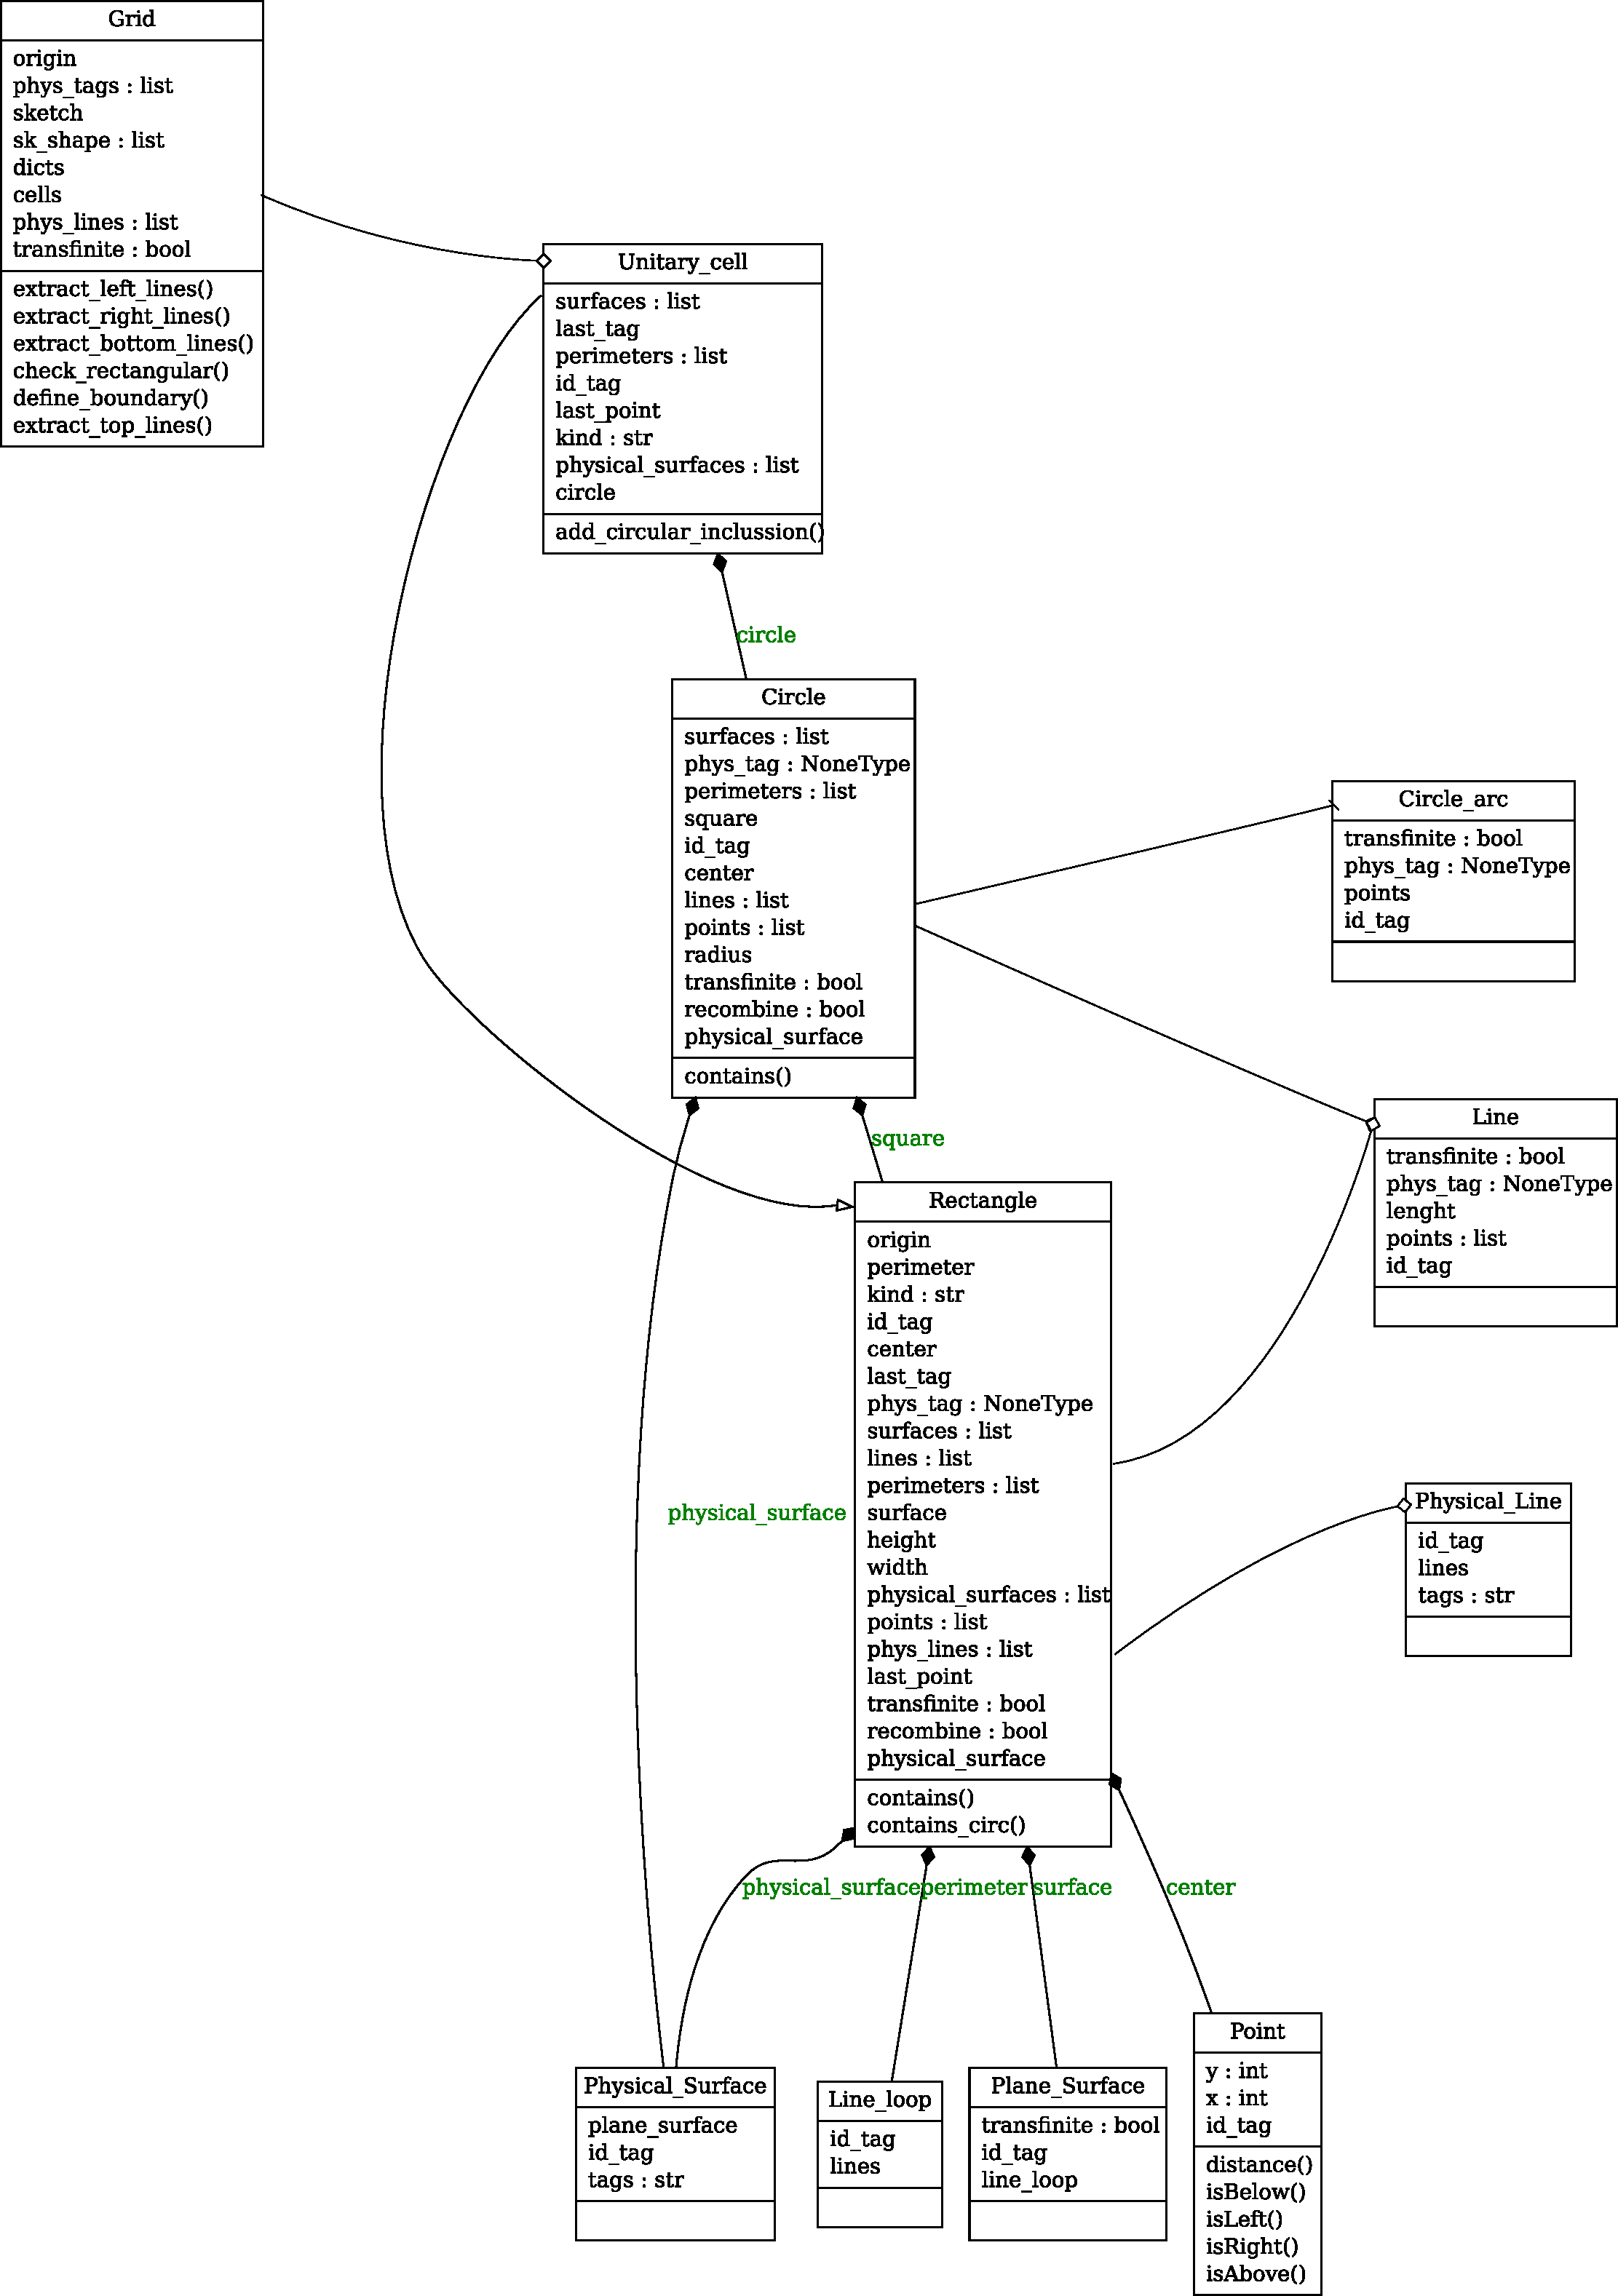
\includegraphics[scale=0.33]{./img/gmsh_library.pdf}
\caption{This diagram shows the classes defined in the module gmsh\_library.py. Classes that are called by a method are connected with lines that end with a black diamonds, inheritance is shown with a white arrow, and classes that are attributes of other classes are connected by white diamonds.}
\label{fig:gmsh_library_classes}
\end{figure}

\section{Paraview}
\begin{quote}``ParaView is an open-source, multi-platform application designed to visualize data sets of size varying from small to very large'' \cite{Henderson2007, ParaviewDoc}.\end{quote}
It is built on top of the Visualization Tool Kit libraries(VTK), so given a \textit{.vtk} file format that contains data one can generate all sorts of graphs and plots from it, and interactively extract quantitative and qualitative information. 
Paraview is used externally in this implementation as the principal post processing tool. The  solution of FE simulations is saved to \textit{.vtk} files by means of writing with routine \verb|write_vtk()| found in library \href{https://github.com/bebopsan/peyeQM/blob/Depuration/Lib/OOPyQM/write.py}{write.py}. All the images from chapter \ref{ch:Results} (except for dispersion plots) were generated using Paraview.



